\documentclass[conference]{IEEEtran}

% \AtBeginDocument{%
% \providecommand\BibTeX{{%
%     Bib\TeX}}}

% \setcopyright{acmlicensed}
% \copyrightyear{2025}
% \acmYear{2025}
% \acmDOI{XXXXXXX.XXXXXXX}
% \acmConference[SC '25]{ACM/IEEE International Conference for High Performance Computing, Networking, Storage and Analysis}{November 16--21, 2025}{St.~Louis, MO}
% \acmISBN{978-1-4503-XXXX-X/2018/06}

\def\BibTeX{{\rm B\kern-.05em{\sc i\kern-.025em b}\kern-.08em
    T\kern-.1667em\lower.7ex\hbox{E}\kern-.125emX}}

\usepackage{cite}
\usepackage{array}
\usepackage{amsmath,amssymb,amsfonts}
\usepackage{algorithm}
\usepackage{algorithmic}
\usepackage{graphicx}
\usepackage{textcomp}
\usepackage{url}
\usepackage{hyperref}
\usepackage[table]{xcolor}

\usepackage{booktabs}
\IfFileExists{tagging.sty}{\usepackage{tagging}}{}
\IfFileExists{ipdps26repro.sty}{\usepackage{ipdps26repro}}{}
% \usepackage{subcaption}
\usepackage{tikz}
\usepackage{listings}
\IfFileExists{ctable.sty}{\usepackage{ctable}}{}
\IfFileExists{subfigure.sty}{\usepackage{subfigure}}{}
\definecolor{dkgreen}{RGB}{0,64,0}
\definecolor{ltgray}{RGB}{245,245,245}
\definecolor{mauve}{RGB}{139,0,139}

\lstset{ %
    language=[90]Fortran,           % the language of the code
    basicstyle=\footnotesize\tt,    % the size of the fonts that are used for the code
    numbers=left,                   % where to put the line-numbers
    numberstyle=\tiny\tt,           % the style that is used for the line-numbers
    stepnumber=1,                   % the step between two line-numbers. If it's 1, each line
                                    % will be numbered
    numbersep=5pt,                  % how far the line-numbers are from the code
    backgroundcolor=\color{ltgray}, % choose the background color. You must add \usepackage{color}
    showspaces=false,               % show spaces adding particular underscores
    showstringspaces=false,         % underline spaces within strings
    showtabs=false,                 % show tabs within strings adding particular underscores
    frame=single,                   % adds a frame around the code
    rulecolor=\color{black},        % if not set, the frame-color may be changed on line-breaks within not-black text (e.g. commens (green here))
    tabsize=2,                      % sets default tabsize to 2 spaces
    captionpos=b,                   % sets the caption-position to bottom
    breaklines=true,                % sets automatic line breaking
    breakatwhitespace=false,        % sets if automatic breaks should only happen at whitespace
%  title=\lstname,                % show the filename of files included with \lstinputlisting;
%                                  % also try caption instead of title
    keywordstyle=\color{blue},          % keyword style
    commentstyle=\color{dkgreen},       % comment style
    stringstyle=\color{mauve},         % string literal style
}

\definecolor{myblue}{RGB}{53, 121, 139}
\definecolor{mygray}{RGB}{240, 255, 240}

% Stage-tag colors for Algorithm 1 (text-contrast variants of the
% fig_stagescale palette).
% Stage colors match the fig_stagescale palette (text-darkened hues):
% Pressure=vermillion, SGS=blue, Derivatives=green, Turbines=purple,
% Projection=rose, Other=orange. Convection has no bar (gray).
\definecolor{stgderiv}{RGB}{0,122,89}    % derivatives  (green)
\definecolor{stgsgs}{RGB}{0,102,160}     % SGS          (blue)
\definecolor{stgconv}{RGB}{100,100,100}  % convection   (gray)
\definecolor{stgturb}{RGB}{128,0,128}    % turbines     (purple)
\definecolor{stgpress}{RGB}{178,72,0}    % pressure     (vermillion)
\definecolor{stgproj}{RGB}{204,102,153}  % projection   (rose)
\definecolor{stgother}{RGB}{150,102,0}   % other        (orange)
% Colored lead words for the time-step walkthrough (Section II).
\newcommand{\stagelead}[2]{{\sffamily\bfseries\color{#1}#2}}
% Right-margin section pointer inside Algorithm 1.
\newcommand{\algptr}[2]{\hfill\mbox{\footnotesize\color{#1}\S\ref{#2}}}


\newcommand{\fix}[1]{\textcolor[rgb]{0.0,0.0,1.0}{#1}}
\newcommand{\tweakedsim}{\raise.17ex\hbox{$\scriptstyle\mathtt{\sim}$}}

% Placeholder box for figures that are not yet generated.
\newcommand{\figplaceholder}[1]{%
  \fbox{\parbox[c][4.5cm][c]{0.92\linewidth}{\centering\footnotesize\fix{#1}}}}

\begin{document}

\title{Accelerating Production-Scale Wind-Farm Large-Eddy Simulation on GPUs}

% \author{\IEEEauthorblockN{Cunyang Wei}
% \IEEEauthorblockA{\textit{Department of Computer Science}\\
% \textit{University of Maryland}\\
% College Park, Maryland 20742 USA\\
% cunyang@umd.edu
% }
% \and
% \IEEEauthorblockN{Abhinav Bhatele}
% \IEEEauthorblockA{\textit{Department of Computer Science}\\
% \textit{University of Maryland}\\
% College Park, Maryland 20742 USA\\
% bhatele@cs.umd.edu
% }
% }

% \renewcommand{\shortauthors}{Wei et al.}

\maketitle

\begin{abstract}
Large-eddy simulation (LES) is the de facto standard for wind-farm aerodynamics
because it directly resolves energy-carrying turbulence in the atmospheric
boundary layer rather than modeling it. LESGO is a widely used open-source
solver for this regime built on pseudo-spectral methods, which carry minimal
numerical dissipation and deliver high accuracy per grid point. LESGO's CPU
implementation, however, suffers from poor parallel scalability, severely
constraining the grid resolution and physical integration times of
production-scale wind-farm simulations. To enable significantly finer resolutions and longer time scales, we
present the porting of LESGO to GPGPUs. For this class of pseudo-spectral
multi-physics solvers with recurring host--device coupling, data movement rather
than kernel throughput governs overall performance. We analyze all host--device
coupling points across the solver and classify them into four treatments. On
this foundation, we propose several optimizations, including chunk pipelining
across serial rank chains, batching many small work items, and heterogeneous
CPU--GPU execution.  Evaluation on a 60-turbine wind farm discretized into 604 million cells
demonstrates a 40$\times$ speedup over the best-performing CPU baseline at
equal node count, rising to 90$\times$ on 64 GPUs, and strong scaling to
128 GPUs on a 1.36 billion cell grid.

\end{abstract}

\begin{IEEEkeywords}
large-eddy simulation, GPU acceleration, \mbox{OpenACC}, 
wind energy, pseudo-spectral methods
\end{IEEEkeywords}

\section{Introduction}
\label{sec:intro}
Wind energy is a central pillar of the global transition to renewable
power, and its continued growth depends on understanding how
turbines interact with the turbulent atmospheric boundary layer (ABL)
and with each other's wakes~\cite{veers2019}. Wake losses in large wind
farms reduce total power output by 10--20\%~\cite{barthelmie2009}, and
mitigating them requires simulating tens of turbines embedded in
kilometers of turbulent atmosphere over hours of physical time.
Large-eddy simulation (LES) resolves these energy-carrying turbulent
motions directly and has become the de facto standard for wind-farm
aerodynamics~\cite{calaf2010, stevens2017}. However, it comes at a steep
computational price when coupling hundreds of millions of grid points to
the long integration times these flows demand.

LESGO~\cite{lesgo-web,bouzeid2005} is a widely used open-source pseudo-spectral
LES solver for ABL and wind-farm flows.  The code has been used for many
different kinds of simulations including wind-farm, rough-surface, canopy,
urban, and wall-bounded flows~\cite{lesgo-publications}. \fix{you need to cite dozens of publications here} Recent work continues
to use LESGO for large wind-farm simulations and public
datasets~\cite{zhu2025jhtdbwind}. \fix{what does use LESGO for public datasets mean?} Its numerical formulation combines Fourier
colocation in the horizontal directions, a scale-dependent Lagrangian dynamic
subgrid-scale (SGS) model~\cite{bouzeid2005}, and actuator-line turbine
coupling~\cite{sorensen2002}. This formulation carries little numerical
dissipation and delivers high accuracy per grid point. Its CPU implementation,
however, saturates node memory bandwidth even at tens of cores and exhausts its
slab decomposition at modest process counts (Section~\ref{sec:bg-impl}), severely
constraining production-scale runs.  Because the scientific fidelity of
turbulent wake simulations relies on capturing long physical integration times,
this performance ceiling directly limits accessible physical time scales.
Porting the solver to GPUs provides a natural path to overcome these
scalability barriers.  \rev{Figure~\ref{fig:wf60-velocity} illustrates the
interacting turbulent wakes in the 60-turbine configuration used for our
production benchmark.} \fix{this statement looks abrupt here, maybe move it to where you talk about dozens of simulations}

Porting large Fortran solvers to GPUs with compiler directives such as
OpenACC is by now well established across weather and climate
models~\cite{lapillonne2014,govett2017nim,norman2015,giorgetta2022,esclapez2025dales},
CFD and turbulence
solvers~\cite{xia2015,otero2019nek,devanna2023uranos}, and production
physics codes in other domains~\cite{caplan2019mas}. By
annotating existing loops instead of rewriting them in a GPU-specific programming
language, this approach keeps a single source tree, which lowers the 
barrier to GPU adoption for large and physics-validated code bases, and lets their user communities maintain the source directly. 
It is especially effective at offloading
compute-intensive kernels, where a self-contained block of arithmetic
moves to the GPU wholesale and improves kernel throughput. For
LESGO, however, the factor that governs performance is
not kernel throughput but data movement.

Pseudo-spectral multiphysics LES has recurring host--device
\emph{coupling points} -- places where host-side code must read or write
device-resident state. They vary widely in how much of the field they
touch and how often, so no single blanket data-placement policy fits
them all. The two data strategies common to directive-based ports both
encounter severe limitations here. (1)~Array mirroring, whether 
wholesale~\cite{esclapez2025dales} or selective~\cite{giorgetta2022}, 
synchronizes data at module boundaries. However, servicing coupling 
points over PCIe still leaves the GPU largely idle.
Moreover, blanket duplication wastes device memory on unconsumed arrays,
restricting per-GPU grid capacity.
(2)~Delegating placement to CUDA managed memory lets the driver migrate
pages on demand, a route that minimizes porting effort and underpins
Fortran standard-parallelism offloading~\cite{caplan2023dc}, yet it
hides traffic from the source code and incurs page-migration overheads 
across a range of GPU workloads~\cite{chien2019um}.
Thus, achieving high performance for LESGO requires developing a
fine-grained data residency strategy tailored to its distinct
host--device coupling points.

In this paper, we present our approach to porting the Fortran solver in LESGO
to GPGPUs. The port preserves the solver's validated physics and brings
production-scale wind-farm LES within practical reach. We begin with an analysis of the 
data movement that measures two established placement strategies \fix{what two strategies?}
on our own code and traces the bottleneck to host--device coupling points.
Guided by this analysis, we analyze all coupling points across the solver,
classify them by host consumer read footprints, and apply four treatments
(gate, slice, relocate, and overlap). \fix{I am not sure what treatements means} Beyond data-residency optimizations, we
apply three other optimizations to overcome remaining structural bottlenecks. We pipeline
independent systems across a serialized rank chain to accelerate the pressure
equation's distributed tridiagonal solve; batch many small work items to
mitigate kernel launch overhead; and hide residual host-side airfoil physics
behind device execution through CPU--GPU heterogeneous execution.

We implement our GPU port in OpenACC using the NVHPC compiler,
and evaluate it on NVIDIA A100 GPUs and H200 GPUs. 
This work makes the following contributions:
\begin{itemize}
\item We present the first ever GPU port of LESGO, covering its full
physics pipeline. To our knowledge, this is the first directive-based 
GPU LES with actuator-line wind-farm coupling at this scale. Our code 
will be open-sourced upon acceptance.
\item We analyze and classify all host--device coupling points by
their host consumer footprints, enforcing minimal data movement through
four distinct treatments (gate, slice, relocate, and overlap).
\item We demonstrate three optimizations on the
solver's coupling-heavy modules: chunk pipelining across serial rank
chains to hide inter-rank communication delays, batching many small
work items to mitigate kernel launch overhead, and CPU--GPU
heterogeneous execution to overlap residual host physics with the GPU
backlog.
\item We evaluate the GPU version at production scale on a 604M-cell, 60-turbine 
wind farm, achieving a 40$\times$ speedup over the fastest CPU baseline.
We also demonstrate scaling up to 128 GPUs on a 1.36 billion-cell grid. 
\end{itemize}


\section{Background}
\label{sec:bg}
This section introduces the numerical formulation and physical models of LESGO and provides a brief overview of the OpenACC programming model.

\subsection{Pseudo-spectral LES formulation}
\label{sec:bg-numerics}

LESGO solves the filtered incompressible Navier--Stokes equations in
rotational form for high-Reynolds-number ABL flow,
%
\begin{equation}
\frac{\partial \tilde{u}_i}{\partial t}
+ \tilde{u}_j\!\left(\frac{\partial \tilde{u}_i}{\partial x_j}
- \frac{\partial \tilde{u}_j}{\partial x_i}\right)
= -\frac{\partial \tilde{p}^{*}}{\partial x_i}
- \frac{\partial \tau_{ij}}{\partial x_j}
+ f_i ,
\label{eq:les}
\end{equation}
%
where $\tilde{u}_i$ is the filtered velocity, $\tilde{p}^{*}$ is the 
modified pressure, $\tau_{ij}$ is the subgrid-scale (SGS) stress tensor, 
and $f_i$ represents body forces, including turbine forcing. The horizontal 
directions are periodic and discretized using Fourier collocation, whereas 
vertical derivatives are evaluated with second-order centered finite 
differences on a staggered grid. Dealiasing of nonlinear terms via the $3/2$ 
rule~\cite{orszag1971} requires forward and inverse FFTs across all velocity 
and vorticity components on a $3/2$-padded grid at every time step. 
Time integration employs a second-order Adams--Bashforth scheme, with
incompressibility enforced by a fractional-step projection. The pressure 
Poisson equation is diagonalized by 2D horizontal FFTs, yielding independent 
1D tridiagonal systems along $z$ for each horizontal wavenumber pair. At 
the lower boundary, an equilibrium log-law stress model~\cite{moeng1984} 
(or optionally an integral wall model~\cite{yang2015iwm}) closes the boundary 
condition. 

Consequently, FFT-based differentiation, dealiased products, and the spectral 
Poisson solve render the computational profile heavily FFT-dominated, 
in contrast to finite-difference atmospheric codes where FFTs are confined to 
the pressure solve~\cite{esclapez2025dales,vanheerwaarden2017}.
Prior GPU accelerations for such FFT-heavy solvers rely on CUDA Fortran,
including ports of finite-difference codes such as CaNS~\cite{costa2018,costa2021}  
and AFiD~\cite{zhu2018afid}, or custom asynchronous redesigns of 
pseudo-spectral codes~\cite{ravikumar2019}.

\subsection{Dynamic SGS and actuator-line turbine models}
\label{sec:bg-physics}

Two physics components dominate both the scientific fidelity and the
computational complexity of wind-farm LES in LESGO.

\textbf{Scale-dependent Lagrangian dynamic SGS (LASD).} An eddy
viscosity closes the SGS stress in Eq.~\ref{eq:les}. The model computes
its coefficient dynamically~\cite{germano1991}, averages it along
fluid-particle trajectories~\cite{meneveau1996}, and recovers scale
dependence through a second test
filter~\cite{porteagel2000,bouzeid2005}. Each
coefficient update applies two spectral test filters to nine tensor
fields (requiring batched 2-D FFTs across all vertical levels) and
advects four accumulator fields along particle back-trajectories via
trilinear interpolation. As the accuracy backbone of LESGO for
heterogeneous ABL flows, this model relies on an irregular memory access
pattern that intertwines filtering, history tracking, and interpolation.
Consequently, mapping this formulation to GPUs presents distinct
challenges compared to conventional local closures that rely
primarily on stencil operations~\cite{esclapez2025dales}, and it
has no counterpart in prior directive-based LES ports.

\textbf{Actuator-line turbine model (ATM).} Each turbine blade is
represented by discrete actuator points that sample the local LES
velocity via trilinear interpolation, look up tabulated airfoil
aerodynamic polars, and project the resulting forces back onto the grid
through a Gaussian convolution kernel~\cite{sorensen2002,martinez2015}.
Simulating multi-turbine farms introduces thousands of moving, off-grid
coupling points that interact with the flow field twice per time step
during velocity sampling and force projection (Section~\ref{sec:opt-atm}). 
Prior GPU-accelerated wind-farm simulation frameworks have largely 
focused on the ExaWind stack~\cite{sharma2024exawind,mullowney2021,kuhn2025amrwind}, 
which comprises second-order finite-volume codes tailored for 
geometry-resolved engineering simulations of finite wind farms. 
In contrast, LESGO addresses a distinct physical regime. Its 
pseudo-spectral discretization introduces zero numerical dissipation, 
enabling turbulence spectra, wake-recovery entrainment, and 
farm-boundary-layer interactions to be resolved without scheme-induced 
contamination. Furthermore, its horizontally periodic formulation 
directly models the fully developed wind-farm boundary layer that 
forms the foundation for atmospheric parameterizations. 

\subsection{GPU acceleration with OpenACC}
\label{sec:bg-openacc}

Early GPU acceleration efforts in atmospheric modeling relied either on 
converting select kernels to CUDA~\cite{michalakes2008,norman2015} or 
on complete solver rewrites~\cite{schalkwijk2012,vanheerwaarden2017}. 
In contrast, directive-based porting has emerged as the practical 
standard for legacy Fortran codebases~\cite{lapillonne2014,govett2017nim,giorgetta2022,esclapez2025dales,otero2019nek}.
OpenACC offloads execution by annotating loop nests with directives
(\texttt{parallel loop}), without altering the underlying source language.
Directives such as \texttt{create} and \texttt{copyin}/\texttt{copyout} 
handle explicit allocation and data movement, \texttt{update} synchronizes 
data on demand, and \texttt{declare create} maintains array residency 
throughout the program lifetime. Kernels compiled with \texttt{default(present)} 
enforce that operand arrays are already resident on the device.
Additionally, the \texttt{async} clause maps operations to asynchronous 
queues to overlap kernel execution, transfers, and library calls, 
with \texttt{wait} clauses ensuring correct data dependency ordering.

Although offloading individual compute loops via OpenACC follows 
well-established conventions, systematically managing data movement 
across a complex multiphysics solver remains the dominant performance 
bottleneck, which we address in Section~\ref{sec:method}.


\section{Baseline Implementation and Motivation}
\label{sec:motivation}
In this section, we first outline the algorithmic structure of a 
single time step of LESGO. Then, we analyze the scaling limits of 
the CPU implementation that motivate our GPU acceleration strategy.

\subsection{Structure of a Time Step}

\label{sec:step}
\begin{algorithm}[h]
\caption{The main time loop of LESGO.}
\label{alg:step}
\begin{algorithmic}[1]
\STATE \texttt{Initialize()}
\FOR{$n = 1, N$}
\STATE \texttt{ComputeDt()}
\STATE \textcolor{stgderiv}{Derivatives()}\algptr{stgderiv}{sec:method-taxonomy}
\STATE \textcolor{stgderiv}{WallStress()}
\STATE \textcolor{stgsgs}{SGS()}
\STATE \hspace{1.3em}\textbf{if} $n \bmod c = 0$ \textbf{then}
\STATE \hspace{2.6em}\textcolor{stgsgs}{UpdateLASDCoefficient()}\algptr{stgsgs}{sec:opt-lasd}
\STATE \hspace{1.3em}\textcolor{stgsgs}{SGSStress()}
\STATE \hspace{1.3em}\textcolor{stgsgs}{StressDivergence()}
\STATE \textcolor{stgconv}{Convection()}
\STATE \textcolor{stgturb}{Turbines()}
\STATE \hspace{1.3em}\textcolor{stgturb}{SampleBladeVelocities()}\algptr{stgturb}{sec:opt-atm}
\STATE \hspace{1.3em}\textcolor{stgturb}{ComputeBladeForces()}\algptr{stgturb}{sec:opt-overlap}
\STATE \hspace{1.3em}\textcolor{stgturb}{SpreadBladeForces()}\algptr{stgturb}{sec:opt-atm}
\STATE \textcolor{stgpress}{AdvanceAB2()}
\STATE \textcolor{stgpress}{Pressure()}
\STATE \hspace{1.3em}\textcolor{stgpress}{PoissonFFT()}
\STATE \hspace{1.3em}\textcolor{stgpress}{PoissonTridiag()}\algptr{stgpress}{sec:opt-tridag}
\STATE \hspace{1.3em}\textcolor{stgpress}{PoissonInvFFT()}
\STATE \textcolor{stgproj}{ProjectVelocity()}
\ENDFOR
\STATE Finalize()
\end{algorithmic}
\end{algorithm}

LESGO follows a conventional time-marching structure. The solver
state comprises the three filtered velocity components of Eq.~\ref{eq:les},
held on the slab-decomposed grid (Section~\ref{sec:bg-impl}). Each
pass of the main time loop in Algorithm~\ref{alg:step} executes three 
primary phases: (1)~assembling the right-hand-side (RHS) convective, 
turbulent, and boundary force terms (lines 3--15), (2)~advancing the 
velocity to an intermediate state via second-order
Adams--Bashforth integration (line 16), and (3)~enforcing incompressibility 
through a Poisson pressure solve and velocity projection step (lines 17--21). 
\texttt{Initialize()} allocates grid arrays, creates FFT plans, and sets up 
turbine geometry at startup, while \texttt{Finalize()} outputs final diagnostics 
and checkpoints. Inside the loop, \texttt{ComputeDt()} dynamically evaluates 
the time step according to the Courant--Friedrichs--Lewy (CFL) stability 
condition, requiring a global \texttt{MPI\_Allreduce} collective across all ranks.
Below, we describe the execution flow of a single time step in detail.

\stagelead{stgderiv}{Derivatives} (lines 4--5). Evaluating the RHS
terms of Eq.~\ref{eq:les} requires velocity gradients, since the SGS
stress depends on the strain-rate tensor and the rotational convective
term on vorticity. Horizontal derivatives are computed spectrally via
2D forward and inverse FFTs on each $x$-$y$ plane, whereas vertical
derivatives use second-order centered differences that read one ghost
plane exchanged with neighbor ranks. This operation forms a uniform,
memory-streaming sweep across the 3D domain. \texttt{WallStress()}
then applies the logarithmic law-of-the-wall model
(Section~\ref{sec:bg-numerics}) to compute surface shear stress on
the boundary ranks.

\stagelead{stgsgs}{SGS} (lines 6--10). Subgrid-scale closure models the 
unresolved turbulent fluxes. Every $c$-th step ($c=5$ in production runs), 
\texttt{UpdateLASDCoefficient()} updates the dynamic Lagrangian scale-dependent (LASD) 
model coefficient $C_s^2$ (Section~\ref{sec:bg-physics}) by applying two 
spectral test filters and advecting dynamic model accumulators along fluid particle 
trajectories, making it the most computationally irregular and memory-bound routine 
in the solver (Section~\ref{sec:opt-lasd}). On every step, \texttt{SGSStress()} 
recalculates the eddy viscosity $\nu_t = C_s^2 \Delta^2 |S|$ using the current 
strain rate and computes the subgrid stress tensor, after which 
\texttt{StressDivergence()} calculates its spatial divergence.

\stagelead{stgconv}{Convection} (line 11). To eliminate aliasing errors 
arising from non-linear convective terms in rotational form, LESGO employs 
the standard $3/2$-rule dealiasing scheme. Each velocity and vorticity 
component undergoes forward and inverse 2D horizontal FFTs on an
expanded ($1.5\times$ padded) grid. Convection represents the most 
FFT-intensive phase of the time step.

\stagelead{stgturb}{Turbines} (lines 12--15). The actuator-line model 
(ALM) represents wind turbine blades as localized aerodynamic force 
sources in Eq.~\ref{eq:les}. \texttt{SampleBladeVelocities()}
samples flow velocities at discrete blade actuator points via 
trilinear 3D spatial interpolation.
\texttt{ComputeBladeForces()} calculates angle of attack, 
relative velocity, and lift/drag forces using lookup tables of empirical 
airfoil polar data. Finally, \texttt{SpreadBladeForces()} projects
these forces back onto surrounding fluid grid points using 3D Gaussian
spatial regularization.

\stagelead{stgpress}{Pressure} (lines 16--20). The intermediate velocity 
field computed by \texttt{AdvanceAB2()} is generally not divergence-free, so 
its divergence acts as the source term for a 3D Poisson equation for
modified pressure. \texttt{PoissonFFT()} transforms the RHS into
horizontal wave space, decoupling horizontal modes into independent
1D vertical tridiagonal linear systems along $z$. \texttt{PoissonTridiag()}
solves these systems across the MPI rank stack (Section~\ref{sec:opt-tridag}),
and \texttt{PoissonInvFFT()} returns the pressure and its horizontal
gradients to physical space, with the vertical gradient evaluated by
finite differencing. Pressure is the only solver stage requiring
fine-grained, globally coupled communication across all vertical ranks.

\stagelead{stgproj}{Projection} (line 21). \texttt{ProjectVelocity()} 
subtracts the pressure gradient from the intermediate velocity to project 
the flow onto solenoidal (divergence-free) space. Finally, point-to-point 
halo exchanges refresh the single-plane ghost layers to prepare velocity 
fields for the subsequent time step's derivative calculations.

\subsection{MPI Slab Decomposition and Scaling Ceiling}
\label{sec:bg-impl}

LESGO is implemented in Fortran~90 and parallelized with MPI using a 1D slab 
decomposition along the vertical ($z$) axis. Each MPI rank owns a contiguous 
block of horizontal $z$-planes spanning the full horizontal domain ($x$-$y$). 
This topology allows 2D horizontal FFTs to execute entirely rank-locally,
completely avoiding expensive 2D domain transposes (\texttt{MPI\_Alltoallv})
required by 2D pencil decompositions~\cite{romero2022}. Primary physical 
fields, including velocity components, modified pressure, and subgrid 
turbulence scalars, are stored as 3D Fortran arrays.

Inter-rank communication in this slab topology follows three main patterns.
First, vertical finite-difference stencils require nearest-neighbor halo 
exchanges of single horizontal planes between adjacent ranks. Second, 
the pressure Poisson solve induces global coupling across all ranks, 
as each vertical tridiagonal system spans the entire domain height after 
horizontal spectral transformation (Section~\ref{sec:opt-tridag}).
Third, small collective reductions execute CFL time-step control, runtime 
diagnostic logging, and per-turbine force aggregation. By avoiding 2D 
domain transposes, this 1D slab decomposition keeps computationally 
intensive horizontal FFTs rank-local at the expense of a globally coupled 
vertical solve.

\begin{figure}[h]
    \centering
    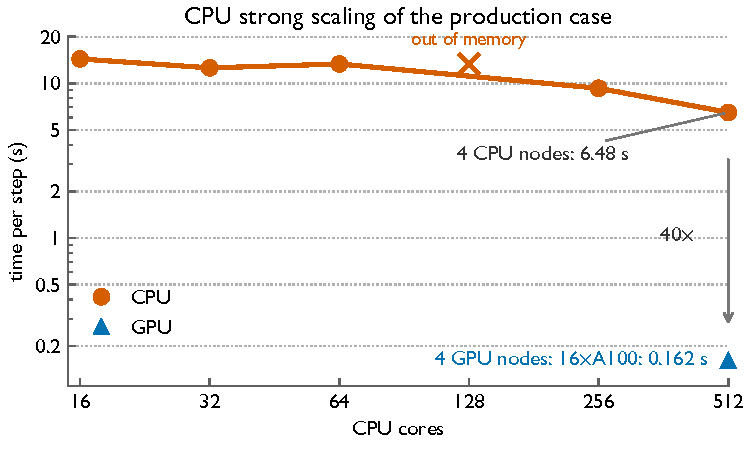
\includegraphics[width=\linewidth]{figs/fig_ceiling.pdf}
    \caption{CPU strong scaling of LESGO on the production wind-farm case of Section~\ref{sec:setup}.}
    \label{fig:ceiling}
\end{figure}
    

On CPU architectures, this design encounters severe scaling limits.
Figure~\ref{fig:ceiling} evaluates the strong scaling of the production
wind-farm case, which simulates 60 turbines on a 472M-cell grid
($3072 \times 384 \times 400$), on Perlmutter CPU nodes with
two 64-core AMD EPYC 7763 (Milan) CPUs each.
As shown in Figure~\ref{fig:ceiling}, the bandwidth-bound solver
saturates a node near 40 of its 128 cores (9.68\,s per step), and
packing 100 ranks onto the same node is counterproductive (11.4\,s).
Scaling out helps only weakly. Two nodes at 200 ranks reach 7.29\,s,
and four nodes at 400 ranks, where the 1D slab decomposition reaches
its structural limit of one vertical plane per rank, plateau at
5.11\,s per step.
At this scaling ceiling, accumulating converged turbulence statistics
requires running hundreds of thousands of time steps. As a result, a single
production simulation takes several hours to days to complete, making
large-scale wind-farm studies computationally impractical. This significant
performance gap motivated our development of the GPU port.


\section{Data Residency Methodology}
\label{sec:method}
This section presents our GPU porting approach, followed by our 
fine-grained data-management strategy designed to minimize host--device 
data movement.

\subsection{Porting Approach}
\label{sec:method-approach}

We ported LESGO using OpenACC directives with the NVHPC compiler and
bound batched cuFFT spectral transforms to the same CUDA streams as the
OpenACC kernels. We chose compiler directives over a low-level CUDA
rewrite because LESGO is an extensive, physics-validated codebase
actively maintained by user community extending the Fortran source.
Directive-based offloading preserves a single source tree in which the
CPU build remains reproducible and acts as our correctness reference.
This approach also aligns with established porting practices in
scientific computing, as demonstrated across atmospheric fluid
models~\cite{esclapez2025dales,lapillonne2014,govett2017nim} and other
production Fortran codebases~\cite{otero2019nek,caplan2019mas}.

The computational pattern across the code is uniform. The solver state
consists of dozens of persistent 3D Fortran arrays of $O(N^3)$ size,
including velocity components, velocity gradients, subgrid-scale (SGS)
stresses, and dealiased spectral scratch fields. Nearly every kernel
sweeps these fields with a triple-nested loop. While this uniformity
simplifies compute offloading, it heightens the penalty for poor data
placement because any unnecessary host--device synchronization transfers
$O(N^3)$ bytes.

\subsection{Data-Movement Bottlenecks}
\label{sec:method-problem}

We now quantify the limitations of the two dominant data-placement
strategies in directive-based ports.

\begin{figure}[h]
  \centering
  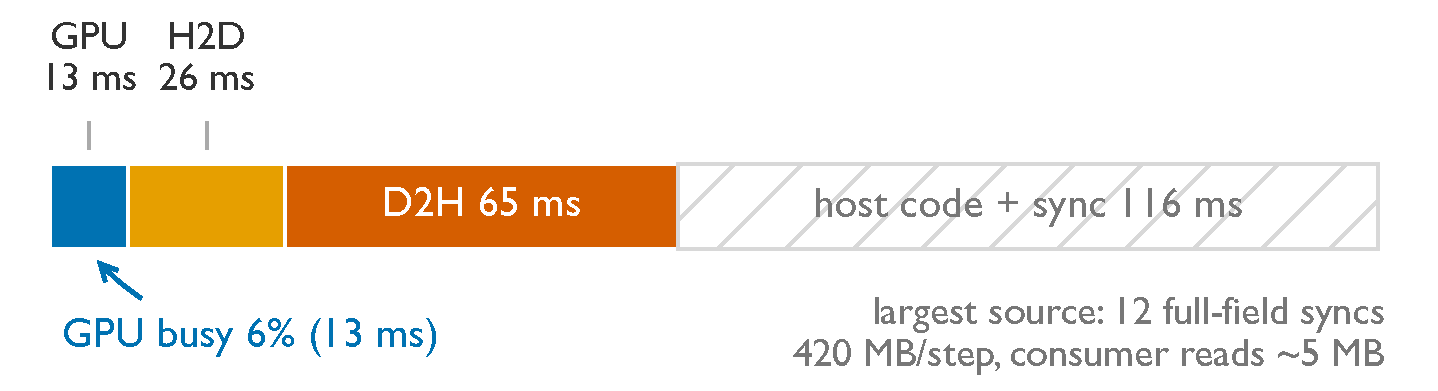
\includegraphics[width=\linewidth]{figs/fig_mirroring.pdf}
  \caption{Time-step breakdown under array mirroring on the reference case ($256^3$ cells, 4 A100 GPUs). Host--device transfers and host-side synchronization leave the GPU 94\% idle.}
  \label{fig:mirroring}
\end{figure}

% \vspace{0.08in}
\textbf{Array Mirroring.} When the solver state fits comfortably in device memory, mirroring every
host array on the device is an effective strategy, as all kernels can
move to the GPU and data returns to the host only for diagnostics and
checkpoints~\cite{esclapez2025dales,giorgetta2022}. LESGO, however,
does not fit this mold for two reasons. First, its state comprises
dozens of $O(N^3)$ fields plus $3/2$-padded spectral scratch, so
duplicating arrays that no kernel reads wastes device memory and increases the number of GPUs a
given grid requires. Second, several routines run slower on the GPU than
on CPUs, and should therefore remain on the host. Mirroring
consequently still requires PCIe transfers wherever these host-resident
routines consume solver state. On our reference configuration ($256^3$
grid with two wind turbines on 4 A100 GPUs), \texttt{Nsight Systems}
profiling reveals that only 13\,ms of a 220\,ms time step is spent on
GPU execution. PCIe transfers and host-side synchronization account for
the remaining 207\,ms, leaving the GPU \textbf{94\% idle}
(Fig.~\ref{fig:mirroring}). The dominant bottleneck is a full-field
synchronization of twelve $O(N^3)$ arrays (420\,MB per step).

% \begin{figure}[h]
% \centering
% 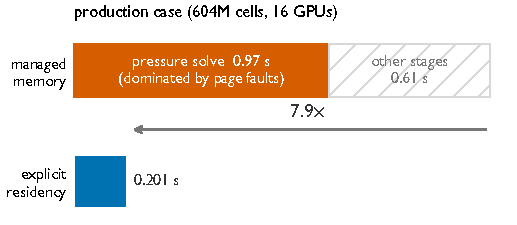
\includegraphics[width=\linewidth]{figs/fig_managed.pdf}
% \caption{Per-step time under CUDA managed memory versus explicit residency on the production case (604M cells, 16 A100 GPUs).}
% \label{fig:managed}
% \end{figure}

\vspace{0.08in}
\textbf{CUDA Managed Memory.} Managed memory minimizes initial porting
effort and underpins Fortran standard-parallelism
offloading~\cite{caplan2023dc}, making it an attractive default for
directive-based ports. However, evaluating CUDA managed memory
(\texttt{-gpu=mem:managed}) on the production benchmark
(Section~\ref{sec:setup}) across 16 A100 GPUs yields limited acceleration. 
Using \texttt{nsys} profiling, we found that
extensive page faults and data migration overheads inherent to
demand-paged unified memory~\cite{chien2019um} severely stall execution.

Both profiles point to the same root cause. After the compute kernels
move to the GPU, certain routines still execute on the host and demand
full-field data transfers to do so. Achieving high GPU efficiency therefore 
requires fine-grained, structure-aware control over data residency and
host--device transfer footprints.

\subsection{Consumer-Driven Explicit Residency}
\label{sec:method-taxonomy}

\begin{table*}[t]
\centering
\caption{Taxonomy of host--device coupling points in a pseudo-spectral
multiphysics LES solver and the data-residency strategies that resolve each class. 
% Naive costs are measured per step on the reference configuration [R] or the production case
% [P].
}
\label{tab:taxonomy}
\footnotesize
\renewcommand{\arraystretch}{1.2}
\rowcolors{2}{gray!12}{white}
\begin{tabular}{@{}
  >{\raggedright\arraybackslash}p{0.8in}
  >{\raggedright\arraybackslash}p{2.35in}
  >{\raggedright\arraybackslash}p{1.05in}
  >{\raggedright\arraybackslash}p{2.25in}@{}}
\toprule
Class & Instance in LESGO & Naive cost per step & Treatment \\
\midrule
Boundary plane & wall-stress model reads $u,v,w$ at the walls &
full fields, 420\,MB & \emph{slice} to wall planes, later
\emph{relocate} \\
Conditional & velocity gradients read by the CPU SGS fallback only &
9 fields, 315\,MB & \emph{gate} on the SGS model choice \\
Spectral mode & pressure zero-wavenumber recurrence (serial in $z$) &
3 full-field round trips & \emph{slice} to the DC column
($\sim$1\,KB) \\
Stale entry & \texttt{copyin} of pressure at solver entry &
34\,MB & \emph{slice} to a seeded ghost plane via \texttt{create} \\
Pipeline state & time integration and projection read $u,v,w$, RHS &
210\,MB & \emph{relocate}, keep the update pipeline
device-resident \\
Actuator & blade sampling and force projection & 2 full-field
crossings & \emph{relocate}, exchange $O(\text{blade points})$
(\S\ref{sec:opt-batch}) \\
Diagnostics & energy, divergence, checkpoint writes & 963\,MB 
& \emph{relocate} reductions, \emph{gate} output
steps \\
Serial chain & tridiagonal Thomas chains spanning ranks &
host-staged relays & \emph{relocate}, pipelined GPU-aware exchange
(\S\ref{sec:opt-tridag}) \\
Host physics & tabulated airfoil polar lookups & serialized 28\,ms
& \emph{overlap} with the GPU backlog (\S\ref{sec:opt-overlap}) \\
\bottomrule
\end{tabular}
\vspace{-0.1in}
\end{table*}

Our port keeps device memory as the primary copy of
every solver field throughout execution, and host routines touch
solver state only at \emph{coupling points}. 
The substance of our strategy is how each coupling point is
treated. We size its transfer by the spatial footprint the host
routine actually accesses. 
We first enforced persistent device residency directly in the source
code. All persistent solver arrays are declared device-resident at
module scope (\texttt{!\$acc declare create}), making residency a
structural property of the data structures. Every GPU kernel asserts
data presence (\texttt{default(present)}). This eliminates routine data
movement and exposes all coupling points for systematic optimization.

We then examined every coupling point along three axes: the spatial
extent the host routine touches (scalar, 1D column, 2D boundary plane,
or 3D subvolume), how often it executes (every step, periodically, or
only under a model option), and its access intent (read-only,
write-only, or read-modify-write). We then group
and classify all coupling points in LESGO into the nine classes listed in
Table~\ref{tab:taxonomy}. For each class, the table gives its concrete
instance in LESGO, the transfer cost that a naive port pays per step, and
the treatment we apply.

Working through the nine classes, we found that four data strategies
suffice to resolve all of them: \emph{gate}, \emph{relocate},
\emph{slice}, and \emph{overlap}. Each exploits a different property of
the coupling point, and we consider them in this order, moving to the
next only when the previous one does not apply.

\vspace{0.08in}
\textbf{Gate} exploits temporal frequency. It applies when the consumer
runs only under a model option or on a subset of steps, such as the
velocity gradients read by the CPU SGS fallback or the fields written at
output steps. The transfer is wrapped in the same guard that controls
the consumer, so it is skipped entirely on steps where the consumer does
not execute.

\vspace{0.08in}
\textbf{Relocate} exploits parallelism in the consumer. If the host
routine parallelizes well, we port it to the GPU so it can read
device-resident data in place. We apply
this to the time-integration and projection pipeline, the diagnostic
reductions, actuator sampling and force projection, and the distributed
tridiagonal chains. 

\vspace{0.08in}
\textbf{Slice} exploits the spatial footprint. It applies when
relocation is not viable because the consumer is inherently serial,
branches irregularly, or performs host-only I/O. 
Those routines stay on the host. We send only the array
section they actually read or write, specified in the \texttt{update
self} and \texttt{update device} directives. For the wall-stress planes,
the pressure DC column, and the ghost plane seeded at solver entry, a
34--420\,MB field transfer becomes a few kilobytes.

\vspace{0.08in}
\textbf{Overlap} is for host work that the first three strategies cannot
remove, such as the tabulated airfoil lookups. Their inputs are known
at a fixed point in the time step, but the computation cannot be
relocated or sliced. We launch the GPU kernels that do not
depend on this work asynchronously and run the host routine while they
execute. The host time is hidden behind device execution
(Section~\ref{sec:opt-overlap}).

Although the instances
reflect LESGO, these classes recur across pseudo-spectral multiphysics
codes, providing a general porting checklist for similar solvers.
To illustrate how these strategies are applied, we present an example below.

\begin{lstlisting}[float=t,linewidth=\columnwidth,
caption={Structure-aware partial transfer for the
pressure DC mode. A 1D column transfer (bottom) replaces full 3D field
synchronization (top).},label={lst:dc}]
! naive: 3 full-field round trips / step
!$acc update self(p)        ! 34 MB
call dc_recurrence(p)       ! touches DC column only
!$acc update device(p)      ! 34 MB

! residency treatment: O(1) traffic
!$acc update self(rH_z(1:2,1,:))  !input column, 1KB
call dc_recurrence_column(p_col)
!$acc update device(p(1:2,1,:))  !output column, 1KB
\end{lstlisting}
  

Consider the spectral special mode from Table~\ref{tab:taxonomy}
(Listing~\ref{lst:dc}). As detailed in
Section~\ref{sec:bg-numerics}, horizontal FFTs reduce the pressure
Poisson equation to independent tridiagonal systems in $z$ for each
horizontal Fourier mode, and the GPU solves all $N^2-1$ non-zero modes
as a single batched system. The zero-wavenumber (DC) mode is singular
and is instead closed by a first-order vertical recurrence. This
recurrence is serial in $z$ and involves only $O(N)$ operations, so a
GPU would execute it slower than a single CPU core, and it remains on
the host. This split matches the slice scenario identified above,
where the compute-intensive batched solve stays on the GPU, the
CPU-friendly serial recurrence stays on the host, and the transfer
shrinks to the consumer footprint.
Our initial port bracketed this lightweight host
computation with full 3D field transfers, resulting in three 34\,MB
round trips per step. The slice instead transfers only the
$\sim$1\,KB input column to the host, evaluates the exact same
recurrence, and pushes the $\sim$1\,KB output column back to the GPU.
As shown in Table~\ref{tab:finalmetrics}, profiling confirms that only 
minimal host--device data transfer remains on the production benchmark. 


\section{Optimizing Coupling-Heavy Components}
\label{sec:opt}
This section presents three optimizations for structural bottlenecks and 
porting practices. Unless noted
otherwise, all performance measurements correspond to the 604M-cell
production case on 16 NVIDIA A100 GPUs (Section~\ref{sec:setup}).

\subsection{Chunk Pipelining across Serial Rank Chains}
\label{sec:opt-tridag}

\begin{figure}[h]
\centering
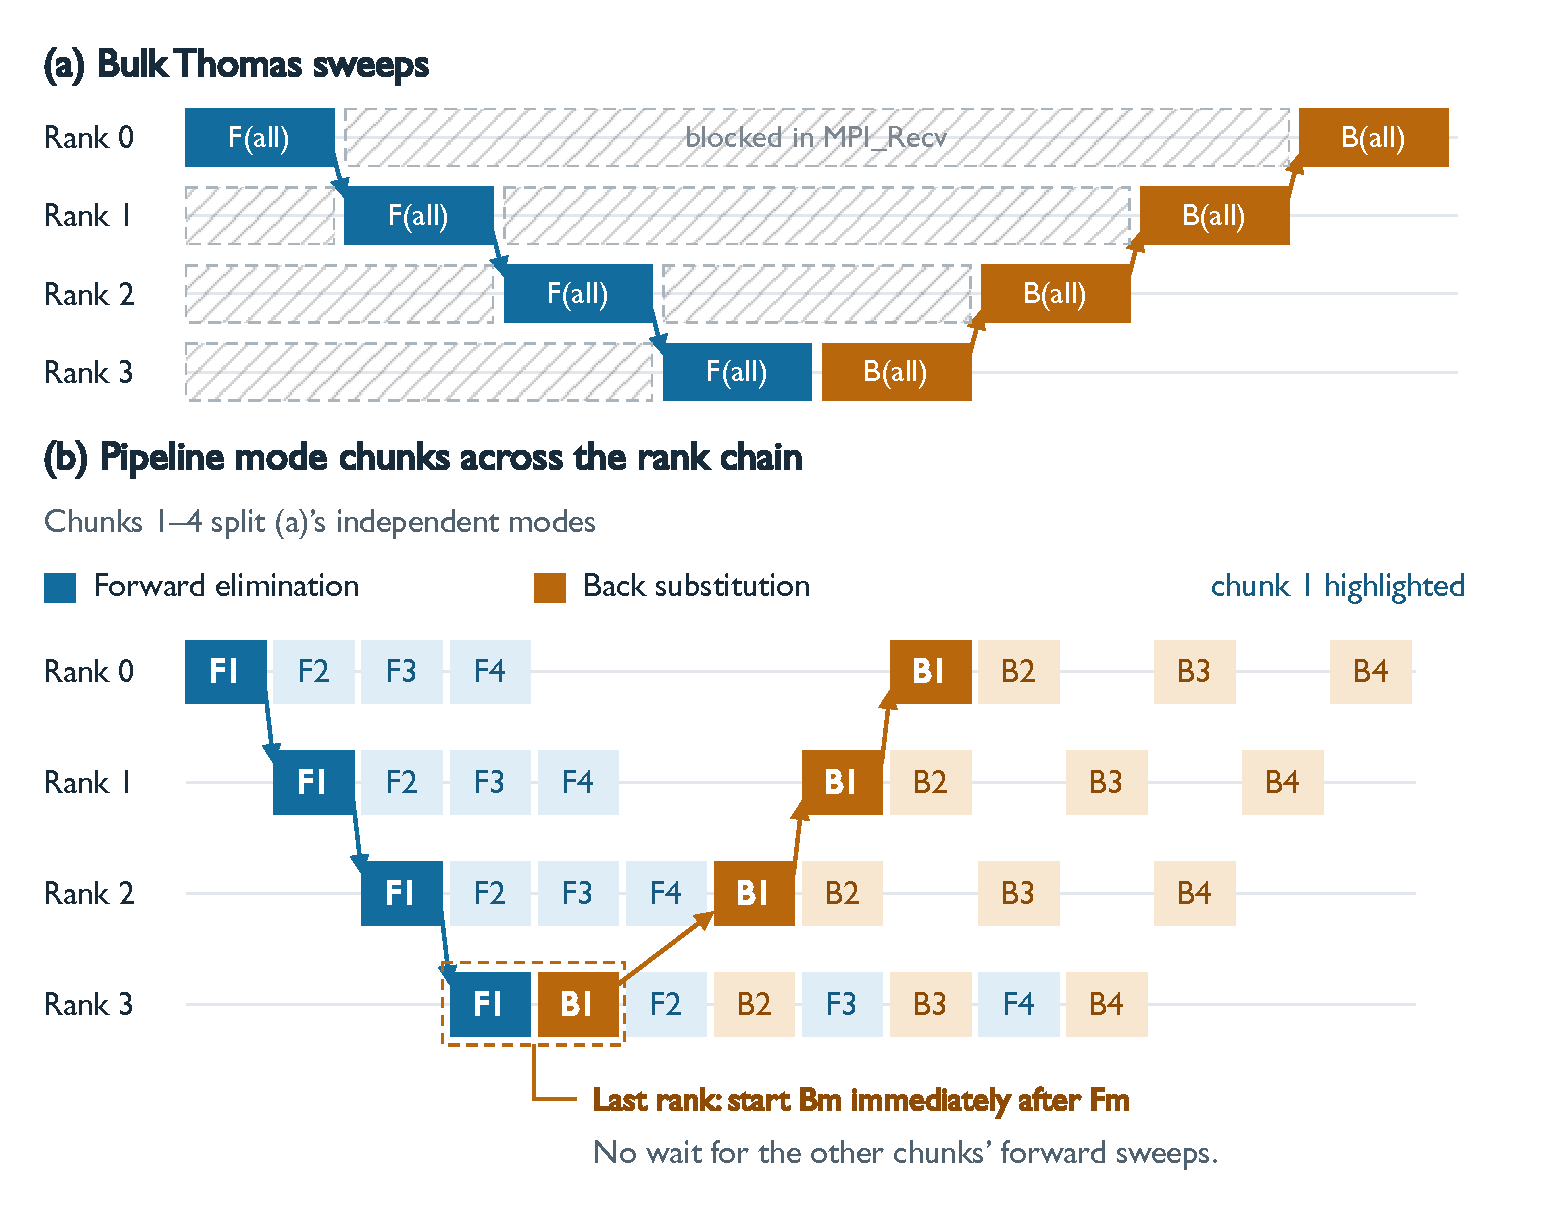
\includegraphics[width=\linewidth]{figs/fig4_lesgo_pipeline.pdf}
\caption{Pipelining the distributed Thomas solve. (a)~Sequential execution leaves ranks idle. (b)~Chunking overlaps forward elimination (blue) with boundary transfers and back substitution (orange).}
\label{fig:tridag}
\end{figure}

In the spectral Poisson solve (\texttt{PoissonTridiag()} in
Algorithm~\ref{alg:step}), independent 1D tridiagonal systems along $z$
arise for each horizontal wavenumber pair. This yields approximately
$590K$ independent systems of 512 unknowns, each distributed across
all 16 ranks in 1D slab domain decomposition. Standard forward
elimination and back substitution in the Thomas algorithm operate
serially along $z$, forcing rank $k$ to idle until rank $k-1$ completes
its forward pass.

To overcome this serialization, we exploit the mutual independence of these systems by partitioning them into $c$ chunks and pipelining the solve~\cite{povitsky1999,povitsky2000} (Fig.~\ref{fig:tridag}). In forward pass, rank $k$ processes chunk $m$, transmits boundary coefficients downstream to rank $k{+}1$, and immediately proceeds to chunk $m{+}1$.
Furthermore, chunking eliminates the global turnaround delay between forward elimination and back substitution. Ordinarily, back substitution must wait for the forward sweep to traverse the entire rank chain. Here, the last rank initiates back substitution for chunk $m$ as soon as its forward pass finishes, overlapping the backward wave of early chunks with the forward sweep of later ones. Unlike
reduced-system libraries that alter the elimination
arithmetic~\cite{laszlo2016,kim2021pascal}, our pipelined approach
leaves the inner Thomas loops untouched, ensuring results equivalence
with the sequential baseline.

\subsection{Batching Many Small Work Items}
\label{sec:opt-batch}

Several solver components decompose into many small, independent work
units. However, each unit is too lightweight to saturate the GPU on its own, 
and has fixed launching overhead. We batch these
units into fewer, larger device operations to amortize that overhead and
improve hardware occupancy.
We demonstrate this strategy with the actuator-line turbine model and the LASD subgrid-scale closure.

For the actuator-line model (\texttt{Turbines()}), 
processing turbines individually repeats device uploads, kernel
launches, synchronizations, and small collective reductions for each
turbine, accumulating over 1,000 \texttt{MPI\_Allreduce} operations per
rank every step. We therefore batch the entire farm into unified device
operations. Blade-point tables for all turbines reside permanently in
device memory. We use a single sampling kernel and a single projection kernel
process all concatenated turbine points, and all reduction quantities
travel in one packed \texttt{MPI\_Allreduce}. Together, these changes
cut per-step kernel launch and collective call counts by an order of
magnitude. The same restructuring also removed repeated device
allocations from the time loop, which
accelerated all other GPU solver stages by 15--18\%.

The Lagrangian scale-dependent (LASD) subgrid-scale model
(\texttt{UpdateLASDCoefficient()} in Algorithm~\ref{alg:step}) demonstrates the
same fragmentation. Each update filters nine 3D tensor fields at two 
test-filter scales: for every horizontal plane, it applies forward 2D FFTs, 
damps selected wavenumber modes, and applies inverse 2D FFTs. 
It also interpolates four accumulator fields to their upstream departure points
$x - u\,\Delta t$. A naive GPU port therefore issues thousands of
single-plane 2D FFTs per update, none large enough to saturate the
device. We therefore batch transforms along the
vertical dimension by promoting 2D scratch planes to 3D arrays, so that
a single batched cuFFT call filters all vertical levels of a field at
once. This consolidation collapses thousands of launches into a few dozen
while exposing enough parallel work per call to fully occupy the device.

\subsection{Heterogeneous CPU--GPU Execution}
\label{sec:opt-overlap}

\begin{figure}[h]
\centering
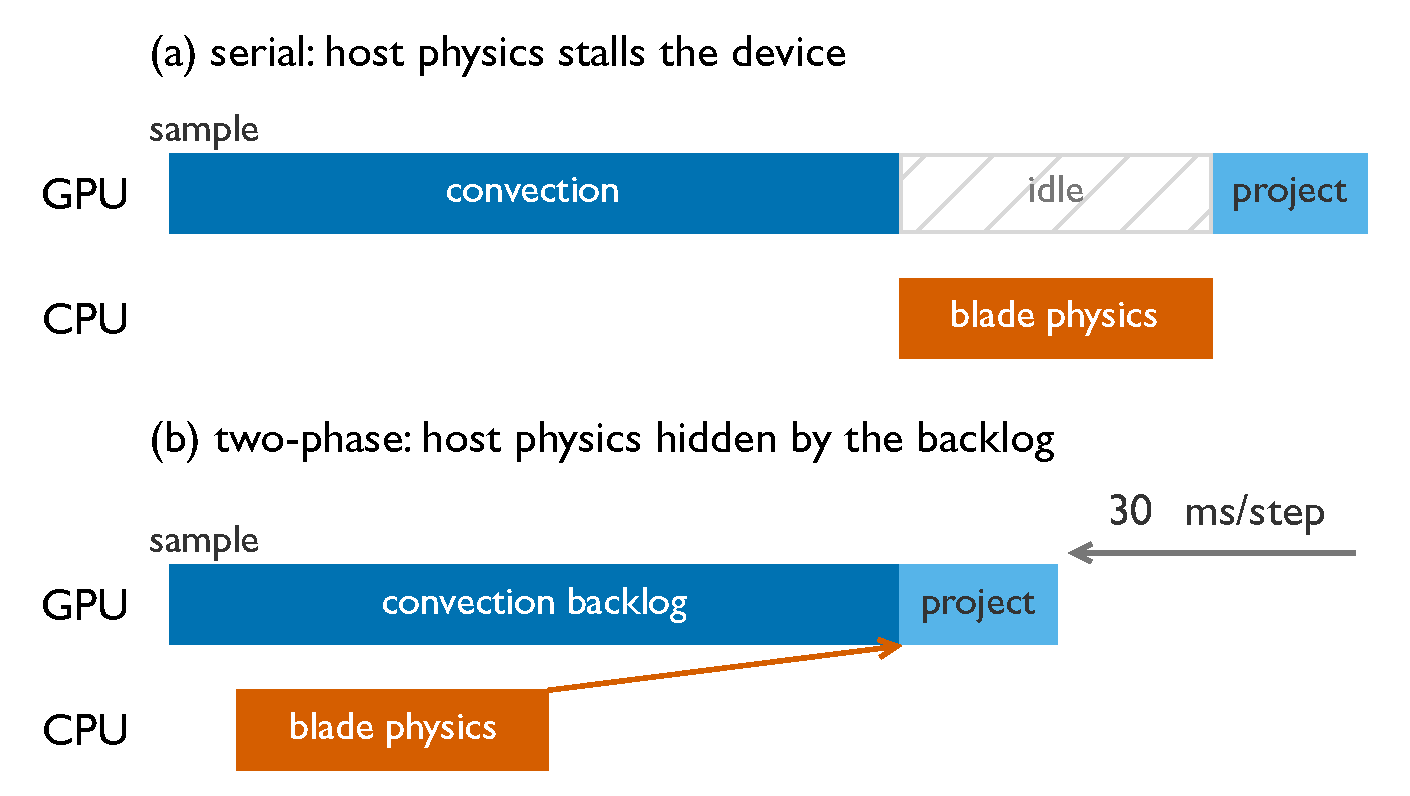
\includegraphics[width=\linewidth]{figs/fig_overlap.pdf}
\caption{Heterogeneous overlap of the actuator-line model.}
\label{fig:overlap}
\end{figure}

We initially ported every computational stage to the GPU, but found that
blade-force evaluation in the actuator-line model
(\texttt{ComputeBladeForces()} in Algorithm~\ref{alg:step}) actually ran
\emph{slower} on the device. 
The production case involves only 10,800 actuator points, far too few
to saturate a GPU. Moreover, each point traverses a data-dependent path
through the airfoil polar lookup, causing warps to serialize.
Kernel-launch and data-transfer overheads therefore exceed the useful
computation. We accordingly keep this routine. 
This decision, however, introduces a new challenge. Host execution
costs $\sim$28\,ms per step, and running it synchronously would leave
the GPU idle at every time step.
We address this by overlapping host computation with concurrent device
work.

Such overlap is feasible because blade-force evaluation only reads
velocities produced at the start of the time step, and its outputs are
not consumed until the force-projection stage later in the step. We
exploit this slack by splitting the actuator-line model into two
decoupled phases around the convection stage
(Fig.~\ref{fig:overlap}). Phase~1 samples blade-point velocities on the
GPU and transfers the compact data packet to the host, returning control
immediately without flushing the device queue. The GPU then proceeds
with convection while the CPU evaluates aerodynamic forces concurrently.
Phase~2 uploads the calculated forces and projects them onto the
Eulerian grid. 
This overlap removes host computation from the critical path, saving
30\,ms per step and raising overall GPU utilization to
\textbf{93\%}. This pattern generalizes to any host routine whose inputs
remain fixed at a known stage of the time step, effectively turning the
CPU into a coprocessor for code that resists GPU offloading.

\subsection{Experiences Porting to Modern GPUs}
\label{sec:opt-impl}

Beyond the optimizations above, we identified three general practices from
our porting effort that apply broadly to directive-based GPU codes.

\vspace{0.08in}
\textbf{Compute Uniformly, Then Patch the Exceptions.} Conditional
logic inside a hot kernel forces every thread in a warp to serialize
along divergent paths, even threads that never take the branch. When
the exceptional points form a lower-dimensional subset of the iteration
space, such as $O(N^2)$ boundary cells versus $O(N^3)$ interior cells,
this penalty is easy to avoid. We use the uniform interior stencil
over the entire domain in a single branch-free kernel with coalesced
accesses, then overwrite boundary values with a second, far smaller
patch kernel. The redundant work is negligible compared to the volume
computation.

\vspace{0.08in}
\textbf{Derive the Parallel Domain from the Data, Not the Loop Nest.}
Translating CPU loop nests directly into GPU kernels tends to inherit
the serial structure of the original code, with poor occupancy and
strided memory traffic. We instead let the data layout
drive the thread decomposition. For regular stencil kernels, we
collapse all spatial loops with the contiguous index innermost so that
warps issue coalesced loads. For work scattered across many small model
instances, we flatten all instances into a single parallel domain of
work items, one thread per item regardless of which instance owns it.

\vspace{0.08in}
\textbf{Align Code Structure with Compiler Offloading Models.} The
NVHPC compiler places small local-array temporaries in thread-private
local memory, which is backed by device DRAM and far slower than
registers. We scalar expand these temporaries so that the compiler can
promote them to registers. 
% We treat the diagnostic output from \texttt{-Minfo=accel} as a mandatory 
% build check to verify that it does so. 
Besides, we found that OpenACC allocates per-thread temporary arrays for every
invocation of Fortran array-valued functions and utility routines. This
means each such call generates device DRAM traffic with substantial
overhead. We therefore manually inline these routines at their call
sites to eliminate the allocation entirely. 

\section{Experimental Setup}
\label{sec:setup}
\textbf{Platforms.} We run our experiments on NERSC Perlmutter~\cite{perlmutter}, 
where each GPU node has four NVIDIA A100 GPUs on a Slingshot-11 interconnect, 
with NVHPC 25.5, CUDA 12.9, cuFFT 11.4, 
and CUDA-aware Cray MPICH 9.1.0. CPU baselines run on the 
Perlmutter's CPU nodes with two 64-core AMD EPYC 7763 (Milan) CPUs each.

\textbf{Cases.} The production case (``wf60'') is a 60-turbine wind
farm of NREL 5-MW reference turbines~\cite{jonkman2009} in a
$10\times6$ array with $7D$ streamwise and $5D$ spanwise spacing
($D=126$\,m), in a $28.2 \times 3.8 \times 2.0$\,km domain discretized
by $3072\times384\times512 \approx 604$M grid points, with the LASD SGS
model, equilibrium wall model, and actuator-line turbines.
Table~\ref{tab:cases} lists the scaling series. Strong scaling runs
the same farm at 512, 768, and 1152 vertical levels (604M, 906M, and
1.36B cells), refining the wall-layer and wake resolution. Weak scaling
fixes the per-GPU grid at three loads and grows the vertical extent with
the GPU count.
We report GPU speedup against the fastest CPU configuration.

\begin{table}[h]
\centering
\caption{Problem sizes of the scaling experiments. Strong scaling keeps
the grid fixed; weak scaling keeps the per-GPU grid fixed.}
\label{tab:cases}
\footnotesize
\setlength{\tabcolsep}{4pt}
\begin{tabular}{@{}lrrl@{}}
\toprule
Grid ($N_x\times N_y\times N_z$) & Cells & Cells/GPU & GPUs \\
\midrule
\multicolumn{4}{@{}l}{\emph{Strong scaling (whole problem)}} \\
$3072\times384\times512$  & 604M  & 37.7M--9.4M  & 16, 32, 64 \\
$3072\times384\times768$  & 906M  & 56.6M--14.2M & 16, 32, 64 \\
$3072\times384\times1152$ & 1.36B & 42.5M--10.6M & 32, 64, 128 \\
\midrule
\multicolumn{4}{@{}l}{\emph{Weak scaling (grid per GPU)}} \\
$3072\times384\times25$ & 118M--1.89B & 29.5M & 4, 8, 16, 32, 64 \\
$512\times512\times40$  & 42M--671M   & 10.5M & 4, 8, 16, 32, 64 \\
$256\times256\times64$  & 16.8M--268M & 4.2M  & 4, 16, 64 \\
\bottomrule
\end{tabular}
\end{table}

\textbf{CPU--GPU backend consistency.}
We first use a small single-turbine case to verify that the CPU and GPU
backends produce consistent LESGO results. Figure~\ref{fig:lesgo-cpu-gpu}
compares matched executions using one NREL 5-MW turbine with a panel-based
actuator-line method and 120 actuator points per blade, with both SGS and
molecular viscosity disabled. Both runs use the same
cold start, $480\times384\times240$ grid, fixed nondimensional time step
$\Delta t=0.0014$, and 1,000 steps. At the common physical time
$t=15.4737$\,s, the transient near-wake fields agree to floating-point
roundoff: the wake-deficit pattern correlation is 1.0, the relative
$L_2$ difference is $1.47\times10^{-13}$, and the maximum normalized axial
velocity difference is $9.00\times10^{-14}$. This test verifies backend
consistency.

\begin{figure*}[t]
\centering
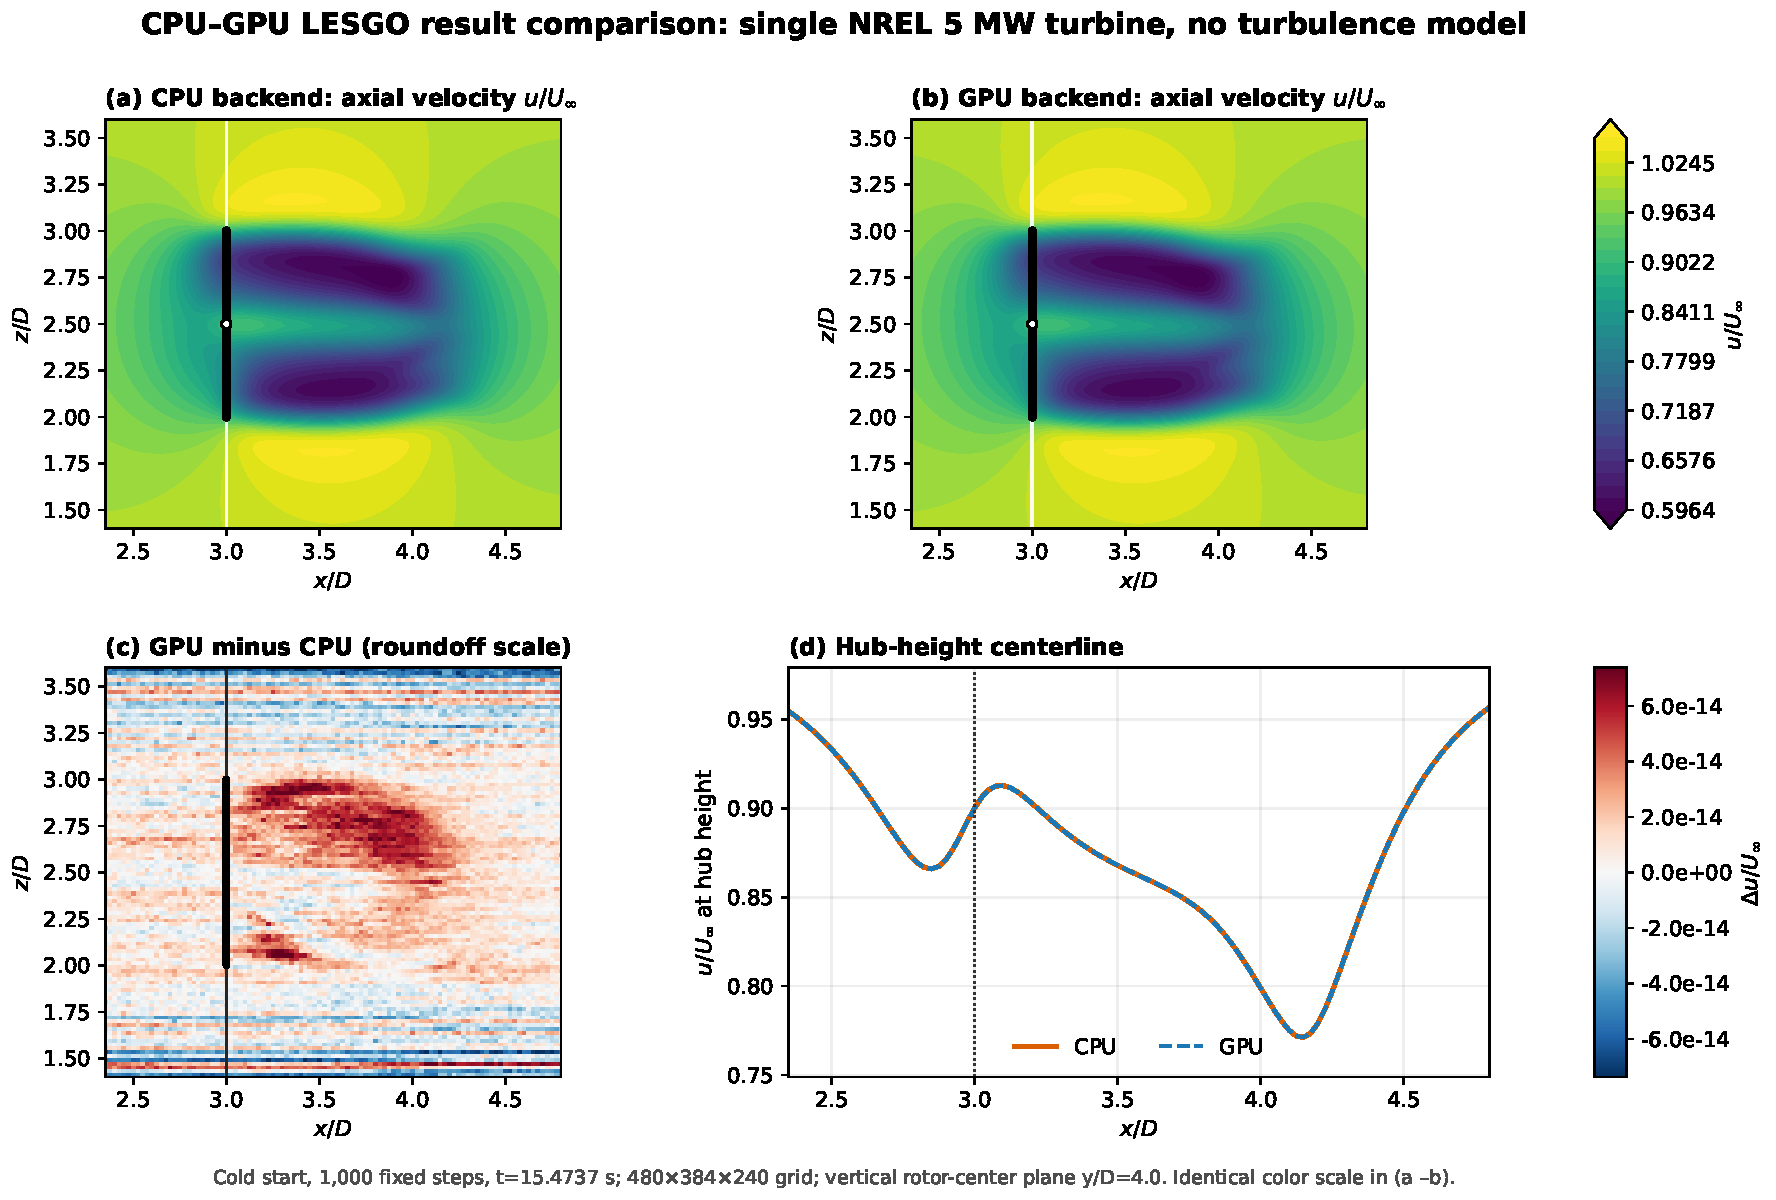
\includegraphics[width=0.96\textwidth]{figs/fig_cpu_gpu_lesgo.pdf}
\caption{Matched CPU--GPU comparison for a 1,000-step LESGO simulation
of one NREL 5-MW turbine at the rated $11.4$\,m\,s$^{-1}$ operating point.
Panels (a) and (b) show normalized axial velocity on the vertical
rotor-center plane using an identical color scale; panel (c) shows the
GPU-minus-CPU difference at roundoff scale; and panel (d) compares the
hub-height centerline profiles. The CPU run used 48 MPI ranks and the GPU run
used two NVIDIA A100 GPUs.}
\label{fig:lesgo-cpu-gpu}
\end{figure*}


\section{Results and Analysis}
\label{sec:results}
This section evaluates solver performance on the production wind-farm
benchmark. We present cumulative speedups, analyze strong and weak
scaling behavior, and demonstrate performance portability across GPU
generations.

\subsection{Production-case performance}
\label{sec:results-prod}

\begin{table}[h]
\centering
\caption{Cumulative speedup of optimizations on 16 A100 GPUs for the
production benchmark (472M cells, 60 turbines) against the fastest
CPU baseline (Fig.~\ref{fig:ceiling}).}
\label{tab:progression}
\footnotesize
\begin{tabular}{@{}lrr@{}}
\toprule
Configuration & s/step & vs.\ CPU \\
\midrule
CPU, fastest configuration (200 ranks)  & 5.09 & 1.0$\times$ \\
Explicit residency (\S\ref{sec:method-taxonomy})
                                       & 1.280 & 4.0$\times$ \\
\;+ actuator-line model on device (\S\ref{sec:opt-atm})
                                       & 0.557 & 9.1$\times$ \\
\;+ chunk-pipelined tridiag.\ solve (\S\ref{sec:opt-tridag})
                                       & 0.294 & 17.3$\times$ \\
\;+ batched actuator-line model (\S\ref{sec:opt-atm})
                                       & 0.186 & 27.4$\times$ \\
\;+ heterogeneous overlap (\S\ref{sec:opt-overlap})
                                       & \textbf{0.157} & \textbf{32$\times$} \\
\midrule
CPU, 200 ranks, with LASD cadence       & \fix{TBD} & 1.0$\times$ \\
Final GPU build, with LASD cadence (\S\ref{sec:opt-lasd})
                                        & 0.196 & $\approx$35$\times$ \\
\bottomrule
\end{tabular}
\end{table}

Table~\ref{tab:progression} summarizes solver progression on the
production benchmark, with each optimization phase corresponding to
its respective section. First, our fine-grained data management 
strategy enables a per-step runtime of 1.28\,s, already $4\times$ 
faster than the fastest CPU configuration. 
Then, relocating the actuator-line coupling onto the device
(\S\ref{sec:opt-atm}) removes the last recurring full-field PCIe
crossings and shortens the step by $2.3\times$. Pipelining the
distributed tridiagonal solve (\S\ref{sec:opt-tridag}) converts the
serialized rank chain of the pressure solver into overlapped chunk
waves for a further $1.9\times$. Batching the 60 turbines into single
kernels and one packed reduction (\S\ref{sec:opt-atm}) removes the
per-instance launch overhead for another $1.6\times$, and hiding the
residual host physics behind the device backlog
(\S\ref{sec:opt-overlap}) contributes the final $1.2\times$. Each
treatment resolves a distinct bottleneck class.
The fully optimized GPU solver achieves 0.157\,s per time step (0.33\,ms
per million cells), representing a $32\times$ speedup over the fastest
CPU configuration. The LASD update (\S\ref{sec:opt-lasd}) fires only every fifth step
at production cadence, so its acceleration appears at full cadence
in the bottom rows of the table rather than inside the per-step
progression. With the model active, step time rises to 0.196\,s
while the speedup widens to $\approx$35$\times$, since the CPU pays
proportionally more for the same physics.
These results demonstrate that our fine-grained data management
methodology and the component optimizations are individually
effective and complementary.




Table~\ref{tab:finalmetrics} profiles execution metrics for the final
build. The GPU remains active for 93\% of
total time step duration, memory transfer volumes confirm zero $O(N^3)$
PCIe data movement during steady-state time marching, and dominant
kernels operate near peak DRAM bandwidth (Fig.~\ref{fig:sol}).

\begin{table}[h]
\centering
\caption{Execution profile of the final port on the production case
(16$\times$A100, \texttt{nsys}/\texttt{ncu}, one time step).}
\label{tab:finalmetrics}
\footnotesize
\begin{tabular}{@{}lr@{}}
\toprule
Metric & Value \\
\midrule
GPU busy fraction & 93\% \\
Host-to-device memcpy volume & \fix{TBD} \\
Device-to-host memcpy volume & \fix{TBD} \\
Memcpy call count & \fix{TBD} \\
Kernel launches & \fix{TBD} \\
Stream synchronizations & \fix{TBD} \\
DRAM bandwidth of dominant kernels & 67--88\% of peak \\
\bottomrule
\end{tabular}
\end{table}

\subsection{Scaling}
\label{sec:results-scaling}

We evaluate strong scaling across three problem sizes, analyze stage-by-stage
execution and kernel efficiency, and examine weak scaling on the
reference setup.

\begin{figure}[h]
\centering
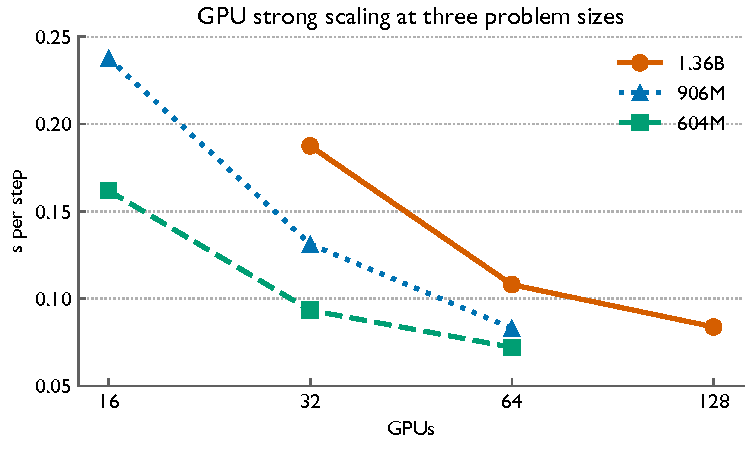
\includegraphics[width=\linewidth]{figs/fig_scaling.pdf}
\caption{Strong scaling of the wind-farm case at three problem
sizes.}
\label{fig:scaling}
\end{figure}

Figure~\ref{fig:scaling} presents strong scaling performance for the
60-turbine wind farm across vertical grid resolutions of 384, 768, and
1152 levels. The solver maintains 95\% parallel efficiency from 16 to
32 GPUs on the 472M-cell grid, 90\% on the 906M-cell grid, and 87\%
from 32 to 64 GPUs on the 1.36B-cell grid, reducing step time from
0.188\,s to 0.108\,s. Scaling extends up to 128 GPUs at 0.084\,s per time
step, achieving a throughput of 16.2 billion cell updates per second.

\begin{figure}[h]
\centering
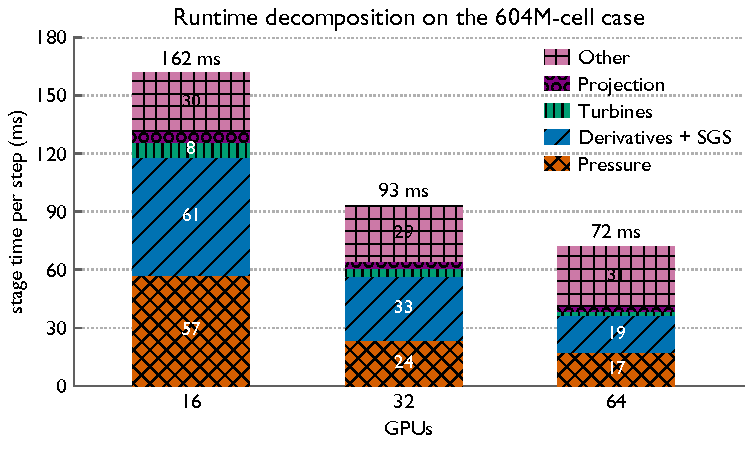
\includegraphics[width=\linewidth]{figs/fig_stagescale.pdf}
\caption{Decomposition of GPU LESGO runtime for the strong scaling cases.}
\label{fig:stagescale}
\end{figure}

To analyze scaling behavior, Figure~\ref{fig:stagescale} decomposes
runtime into individual solver stages from Algorithm~\ref{alg:step}. Each
GPU stage scales predictably with per-device workload. From 16 to 64
GPUs, SGS execution time decreases from 33\,ms to 9\,ms, derivative
evaluation drops from 24\,ms to 6\,ms, and the pressure solver exhibits
superlinear scaling up to 32 GPUs as thinner slab dimensions deepen the
tridiagonal pipeline (Section~\ref{sec:opt-tridag}). At high GPU
counts, execution time is bounded by a constant overhead of
approximately 50\,ms across 64 to 128 GPUs. This overhead primarily
stems from the \texttt{Other} stage, which includes latency-bound collectives such
as global CFL reductions to handle turbine-forcing load imbalances,
along with a constant kernel launch budget measuring 31\,ms across all
runs. The remaining overhead reflects the minimal latency floor of the
tridiagonal pipeline.

Overall step time thus follows a model composed of scalable GPU compute
and a fixed latency term. Maintaining roughly 20 million grid cells
per GPU ensures that scalable computation dominates total execution,
preserving high parallel efficiency. Consequently, parallel efficiency
at a fixed GPU count increases with problem size, directly benefiting
production-scale simulations. This fixed latency term represents an
essential algorithmic baseline. Global CFL reductions enforce adaptive
time stepping correctness, mandatory kernel dispatches persist after
batching thousands of small launches (Section~\ref{sec:opt-atm} and
Section~\ref{sec:opt-lasd}), and the pipeline latency floor represents
the physical limit of serial vertical operations (Section~\ref{sec:opt-tridag}).
Because computational kernels operate near peak DRAM bandwidth
(Fig.~\ref{fig:sol}), remaining overheads are governed by hardware
interconnect and host runtime latencies.

\begin{figure}[h]
\centering
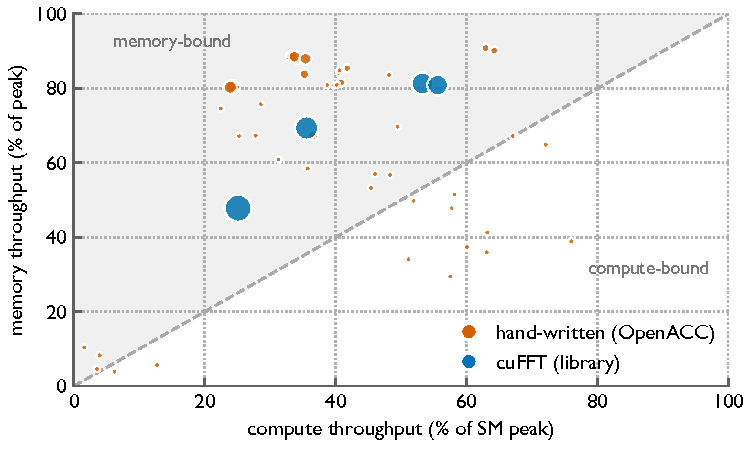
\includegraphics[width=\linewidth]{figs/fig_sol.pdf}
\caption{Nsight Compute speed-of-light utilization of every kernel in
one production step (16$\times$A100, rank 0). Point area is
proportional to each kernel's share of profiled time.}
\label{fig:sol}
\end{figure}

Nsight Compute profiling demonstrates that every major kernel
operates near the hardware's memory-bandwidth roof
(Fig.~\ref{fig:sol}). Custom field kernels achieve 67--88\% of peak DRAM
bandwidth at 24--37\% of peak compute throughput, while batched cuFFT
kernels reach 48--81\% of peak memory bandwidth. As expected for
pseudo-spectral methods, overall performance is governed by GPU memory
bandwidth.

\begin{figure}[h]
\centering
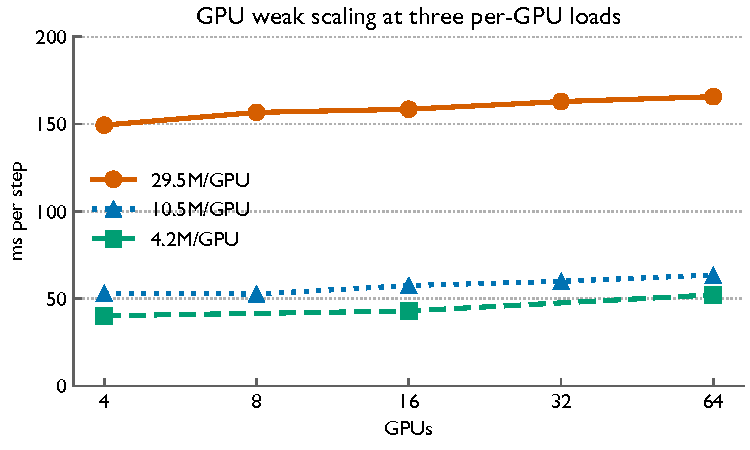
\includegraphics[width=\linewidth]{figs/fig_scaling_weak.pdf}
\caption{Weak scaling ($256\times256\times64$ points per GPU).}
\label{fig:weakscaling}
\end{figure}

Weak scaling benchmarks on the reference setup (Fig.~\ref{fig:weakscaling},
fixed at $256\times256\times64$ grid points per GPU) demonstrate 83\%
parallel efficiency up to 32 GPUs (increasing from 39.5\,ms to 47.8\,ms
per step) and 72\% efficiency at 64 GPUs (54.8\,ms per step). Stage
profiling indicates that derivative evaluation, SGS modeling, and
convection runtimes remain constant within 1\%, while pressure solve
time increases moderately due to tridiagonal chain extension across
deeper slab stacks. The 1D slab decomposition keeps all FFT transforms
rank-local, avoiding all-to-all communication overheads.

While a 2D pencil decomposition could extend rank limits further, the
1D slab structure fully satisfies our target physics. LESGO does not
pursue ever-larger wind-farm domains. It instead resolves the
turbulence physics of horizontally periodic atmospheric boundary
layers and their interaction with turbine arrays, where the grid is
set by the scales of turbulent motion rather than by domain extent.
The demonstrated range (1.36 billion cells at 87\% parallel
efficiency across 128 GPUs) therefore provides ample computational
support for production research of this class. For this reason, 
retaining the 1D slab
decomposition avoids an unnecessary architectural rewrite while
preserving structural alignment with the community-maintained CPU
codebase.

\subsection{Portability and capacity}
\label{sec:results-portability}

\begin{table}[h]
\centering
\caption{Cross-hardware behavior of the production case (no retuning).
A100 rows are Perlmutter, and H200 rows are NCSA Delta.}
\label{tab:portability}
\footnotesize
\begin{tabular}{@{}lrrl@{}}
\toprule
GPU & s/step & Mcell/s/GPU \\
\midrule
16$\times$A100 & 0.157 & 188 \\
8$\times$H200  & 0.250 & 236 \\
\bottomrule
\end{tabular}
\end{table}

Table~\ref{tab:portability} evaluates solver portability across GPU
hardware architectures without code retuning. Device memory capacity
serves as the primary portability metric for pseudo-spectral workloads.
The 472M-cell production case requires 16 A100 GPUs, whereas eight
141\,GB H200 GPUs execute the same simulation with half the GPU count.
Furthermore, H200 GPUs deliver a 26\% higher per-device throughput
(236 versus 188 million cell updates per second per GPU) because
halving the rank count doubles slab thickness and reduces inter-rank halo
and pipeline communication. Consequently, GPU memory capacity directly
enhances both simulation scale and computational efficiency in
slab-decomposed spectral solvers.

\subsection{Time to science}
\label{sec:results-science}
\fix{add science results here}

\begin{figure}[h]
\centering
\figplaceholder{figure from the production science run}
\caption{production simulation. }
\label{fig:wake}
\end{figure}


\section{Conclusion}
\label{sec:conclusion}
We presented the first GPU port of LESGO, a pseudo-spectral wind-farm
large-eddy simulation solver comprising nearly 70{,}000 lines of
Fortran code. We demonstrated that porting such a legacy codebase 
requires a fine-grained data-management strategy. Therefore, we 
identified four data-management operations, 
and classified every host--device coupling point in LESGO
into these solutions. In addition, we demonstrated three
optimizations, including chunk pipelining across serial rank chains,
batching many small work items, and CPU--GPU heterogeneous overlap,
raising overall GPU utilization to 93\%. We believe these
optimizations extend beyond LESGO to broader multiphysics solvers. 
On a production-scale benchmark, our GPU implementation delivers up to
40$\times$ speedup over the fastest CPU baseline. 
We expect this to shorten a full production campaign of a 
60-turbine wind farm from months to days.


% \section*{Acknowledgment}
% \input{ack}

\bibliographystyle{IEEEtran}
\bibliography{./bib/cite,./bib/pssg}

\end{document}
